\chapter{Release}\label{record-274}

\noindent{\footnotesize\color{BookMuted}\path{docs/release.md}\par}\smallskip

\emph{Bijou's official release process}

Bijou adopts the spirit of the older ``Universal Release Pre-Flight'' prompt, but this file is now the repo-native source of truth.

When this document and a generic release prompt disagree, this document wins.

\section{Scope}\label{record-274-scope}

Bijou is currently:

\begin{itemize}
\tightlist
\item
  an npm workspace monorepo
\item
  lock-step versioned across all workspace packages
\item
  tag-driven for release automation
\item
  GitHub Actions driven for publish, release notes, and GitHub Release creation
\item
  npm-only for registry publishing; JSR is not part of the current release surface
\end{itemize}

\section{Operator Flow}\label{record-274-operator-flow}

The older generic release prompt mixed together two different kinds of checks:

\begin{itemize}
\tightlist
\item
  repo guards that must pass \textbf{before} any release mutation happens
\item
  validation gates that run \textbf{after} versions and release docs are updated
\end{itemize}

Bijou keeps that distinction explicit.

Phase 1 is an operator preflight. It proves that the repository is in a safe starting state.

\texttt{r\allowbreak{}e\allowbreak{}l\allowbreak{}e\allowbreak{}a\allowbreak{}s\allowbreak{}e\allowbreak{}:\allowbreak{}r\allowbreak{}e\allowbreak{}a\allowbreak{}d\allowbreak{}i\allowbreak{}n\allowbreak{}e\allowbreak{}s\allowbreak{}s} belongs later. By the time it runs, the worktree is supposed to contain the version bump, changelog edit, and README update. That is why \texttt{r\allowbreak{}e\allowbreak{}l\allowbreak{}e\allowbreak{}a\allowbreak{}s\allowbreak{}e\allowbreak{}:\allowbreak{}r\allowbreak{}e\allowbreak{}a\allowbreak{}d\allowbreak{}i\allowbreak{}n\allowbreak{}e\allowbreak{}s\allowbreak{}s} is the validation gauntlet, not the ``clean worktree'' guard.

\section{Non-Negotiable Rules}\label{record-274-non-negotiable-rules}

\begin{enumerate}
\def\labelenumi{\arabic{enumi}.}
\tightlist
\item
  Run release phases in order.
\item
  Abort on the first hard failure.
\item
  Never claim a release succeeded unless the tag, workflows, and npm registry state were directly verified.
\item
  Never create a release tag from a dirty worktree.
\item
  Never create a release tag from a branch other than \texttt{m\allowbreak{}a\allowbreak{}i\allowbreak{}n}.
\item
  Never create a release tag from a \texttt{m\allowbreak{}a\allowbreak{}i\allowbreak{}n} that is ahead of or behind \texttt{o\allowbreak{}r\allowbreak{}i\allowbreak{}g\allowbreak{}i\allowbreak{}n\allowbreak{}/\allowbreak{}m\allowbreak{}a\allowbreak{}i\allowbreak{}n}.
\item
  Use repo-native tooling:

  \begin{itemize}
  \tightlist
  \item
    version bump: \texttt{n\allowbreak{}p\allowbreak{}m\allowbreak{} \allowbreak{}r\allowbreak{}u\allowbreak{}n\allowbreak{} \allowbreak{}v\allowbreak{}e\allowbreak{}r\allowbreak{}s\allowbreak{}i\allowbreak{}o\allowbreak{}n\allowbreak{} \allowbreak{}X\allowbreak{}.\allowbreak{}Y\allowbreak{}.\allowbreak{}Z}
  \item
    metadata check: \texttt{n\allowbreak{}p\allowbreak{}m\allowbreak{} \allowbreak{}r\allowbreak{}u\allowbreak{}n\allowbreak{} \allowbreak{}r\allowbreak{}e\allowbreak{}l\allowbreak{}e\allowbreak{}a\allowbreak{}s\allowbreak{}e\allowbreak{}:\allowbreak{}p\allowbreak{}r\allowbreak{}e\allowbreak{}f\allowbreak{}l\allowbreak{}i\allowbreak{}g\allowbreak{}h\allowbreak{}t}
  \item
    local gauntlet: \texttt{n\allowbreak{}p\allowbreak{}m\allowbreak{} \allowbreak{}r\allowbreak{}u\allowbreak{}n\allowbreak{} \allowbreak{}r\allowbreak{}e\allowbreak{}l\allowbreak{}e\allowbreak{}a\allowbreak{}s\allowbreak{}e\allowbreak{}:\allowbreak{}r\allowbreak{}e\allowbreak{}a\allowbreak{}d\allowbreak{}i\allowbreak{}n\allowbreak{}e\allowbreak{}s\allowbreak{}s}
  \item
    CI dry-run: \texttt{.\allowbreak{}g\allowbreak{}i\allowbreak{}t\allowbreak{}h\allowbreak{}u\allowbreak{}b\allowbreak{}/\allowbreak{}w\allowbreak{}o\allowbreak{}r\allowbreak{}k\allowbreak{}f\allowbreak{}l\allowbreak{}o\allowbreak{}w\allowbreak{}s\allowbreak{}/\allowbreak{}r\allowbreak{}e\allowbreak{}l\allowbreak{}e\allowbreak{}a\allowbreak{}s\allowbreak{}e\allowbreak{}-\allowbreak{}d\allowbreak{}r\allowbreak{}y\allowbreak{}-\allowbreak{}r\allowbreak{}u\allowbreak{}n\allowbreak{}.\allowbreak{}y\allowbreak{}m\allowbreak{}l}
  \item
    tag publish: \texttt{.\allowbreak{}g\allowbreak{}i\allowbreak{}t\allowbreak{}h\allowbreak{}u\allowbreak{}b\allowbreak{}/\allowbreak{}w\allowbreak{}o\allowbreak{}r\allowbreak{}k\allowbreak{}f\allowbreak{}l\allowbreak{}o\allowbreak{}w\allowbreak{}s\allowbreak{}/\allowbreak{}p\allowbreak{}u\allowbreak{}b\allowbreak{}l\allowbreak{}i\allowbreak{}s\allowbreak{}h\allowbreak{}.\allowbreak{}y\allowbreak{}m\allowbreak{}l}
  \end{itemize}
\item
  Respect lock-step versioning across the workspace.
\item
  Prepare releases on a branch, merge through a PR, and tag only the exact merged \texttt{o\allowbreak{}r\allowbreak{}i\allowbreak{}g\allowbreak{}i\allowbreak{}n\allowbreak{}/\allowbreak{}m\allowbreak{}a\allowbreak{}i\allowbreak{}n} commit.
\end{enumerate}

\section{Registry Setup}\label{record-274-registry-setup}

Bijou publishes public packages to npm through GitHub Actions and npm trusted publishing. Do not store npm automation tokens in GitHub secrets.

For a new public workspace package, first publish one version manually from the package directory so npm has a package record:

\begin{CodeBlock}
npm login
NPM_CONFIG_PROVENANCE=false npm publish --access public
\end{CodeBlock}

The seed publish is deliberately non-provenance because it runs outside the trusted GitHub Actions OIDC environment. After the trusted publisher is configured, automated releases should publish with provenance through \texttt{p\allowbreak{}u\allowbreak{}b\allowbreak{}l\allowbreak{}i\allowbreak{}s\allowbreak{}h\allowbreak{}.\allowbreak{}y\allowbreak{}m\allowbreak{}l}.

Then configure the npm package trusted publisher:

\begin{itemize}
\tightlist
\item
  Organization/user: \texttt{f\allowbreak{}l\allowbreak{}y\allowbreak{}i\allowbreak{}n\allowbreak{}g\allowbreak{}r\allowbreak{}o\allowbreak{}b\allowbreak{}o\allowbreak{}t\allowbreak{}s}
\item
  Repository: \texttt{b\allowbreak{}i\allowbreak{}j\allowbreak{}o\allowbreak{}u}
\item
  Workflow filename: \texttt{p\allowbreak{}u\allowbreak{}b\allowbreak{}l\allowbreak{}i\allowbreak{}s\allowbreak{}h\allowbreak{}.\allowbreak{}y\allowbreak{}m\allowbreak{}l}
\item
  GitHub environment: \texttt{n\allowbreak{}p\allowbreak{}m}
\end{itemize}

The GitHub \texttt{n\allowbreak{}p\allowbreak{}m} environment does not need registry secrets for trusted publishing. Keep the package manifest \texttt{p\allowbreak{}u\allowbreak{}b\allowbreak{}l\allowbreak{}i\allowbreak{}s\allowbreak{}h\allowbreak{}C\allowbreak{}o\allowbreak{}n\allowbreak{}f\allowbreak{}i\allowbreak{}g\allowbreak{}.\allowbreak{}p\allowbreak{}r\allowbreak{}o\allowbreak{}v\allowbreak{}e\allowbreak{}n\allowbreak{}a\allowbreak{}n\allowbreak{}c\allowbreak{}e} setting aligned with the publish workflow so npm records provenance for automated releases.

JSR setup from other projects does not apply to Bijou today. If Bijou later adds \texttt{j\allowbreak{}s\allowbreak{}r\allowbreak{}.\allowbreak{}j\allowbreak{}s\allowbreak{}o\allowbreak{}n}, JSR package records, and a JSR publish workflow, update this runbook and the automation in the same PR.

\section{Release Law}\label{record-274-release-law}

No public release tag may be created unless all automated and human evidence gates below are satisfied. A failed automated gate blocks the release. A human review gate blocks the release until the release evidence packet records either the required update or an explicit ``reviewed, no change'' disposition.

\subsection{Automated Evidence Gates}\label{record-274-automated-evidence-gates}

The current executable gates are \texttt{n\allowbreak{}p\allowbreak{}m\allowbreak{} \allowbreak{}r\allowbreak{}u\allowbreak{}n\allowbreak{} \allowbreak{}r\allowbreak{}e\allowbreak{}l\allowbreak{}e\allowbreak{}a\allowbreak{}s\allowbreak{}e\allowbreak{}:\allowbreak{}p\allowbreak{}r\allowbreak{}e\allowbreak{}f\allowbreak{}l\allowbreak{}i\allowbreak{}g\allowbreak{}h\allowbreak{}t}, \texttt{n\allowbreak{}p\allowbreak{}m\allowbreak{} \allowbreak{}r\allowbreak{}u\allowbreak{}n\allowbreak{} \allowbreak{}r\allowbreak{}e\allowbreak{}l\allowbreak{}e\allowbreak{}a\allowbreak{}s\allowbreak{}e\allowbreak{}:\allowbreak{}r\allowbreak{}e\allowbreak{}a\allowbreak{}d\allowbreak{}i\allowbreak{}n\allowbreak{}e\allowbreak{}s\allowbreak{}s}, \texttt{.\allowbreak{}g\allowbreak{}i\allowbreak{}t\allowbreak{}h\allowbreak{}u\allowbreak{}b\allowbreak{}/\allowbreak{}w\allowbreak{}o\allowbreak{}r\allowbreak{}k\allowbreak{}f\allowbreak{}l\allowbreak{}o\allowbreak{}w\allowbreak{}s\allowbreak{}/\allowbreak{}r\allowbreak{}e\allowbreak{}l\allowbreak{}e\allowbreak{}a\allowbreak{}s\allowbreak{}e\allowbreak{}-\allowbreak{}d\allowbreak{}r\allowbreak{}y\allowbreak{}-\allowbreak{}r\allowbreak{}u\allowbreak{}n\allowbreak{}.\allowbreak{}y\allowbreak{}m\allowbreak{}l}, \texttt{.\allowbreak{}g\allowbreak{}i\allowbreak{}t\allowbreak{}h\allowbreak{}u\allowbreak{}b\allowbreak{}/\allowbreak{}w\allowbreak{}o\allowbreak{}r\allowbreak{}k\allowbreak{}f\allowbreak{}l\allowbreak{}o\allowbreak{}w\allowbreak{}s\allowbreak{}/\allowbreak{}t\allowbreak{}a\allowbreak{}g\allowbreak{}-\allowbreak{}g\allowbreak{}u\allowbreak{}a\allowbreak{}r\allowbreak{}d\allowbreak{}.\allowbreak{}y\allowbreak{}m\allowbreak{}l}, and \texttt{.\allowbreak{}g\allowbreak{}i\allowbreak{}t\allowbreak{}h\allowbreak{}u\allowbreak{}b\allowbreak{}/\allowbreak{}w\allowbreak{}o\allowbreak{}r\allowbreak{}k\allowbreak{}f\allowbreak{}l\allowbreak{}o\allowbreak{}w\allowbreak{}s\allowbreak{}/\allowbreak{}p\allowbreak{}u\allowbreak{}b\allowbreak{}l\allowbreak{}i\allowbreak{}s\allowbreak{}h\allowbreak{}.\allowbreak{}y\allowbreak{}m\allowbreak{}l}.

The release policy requires these checks, even where the current implementation still relies on operator verification:

\begin{center}
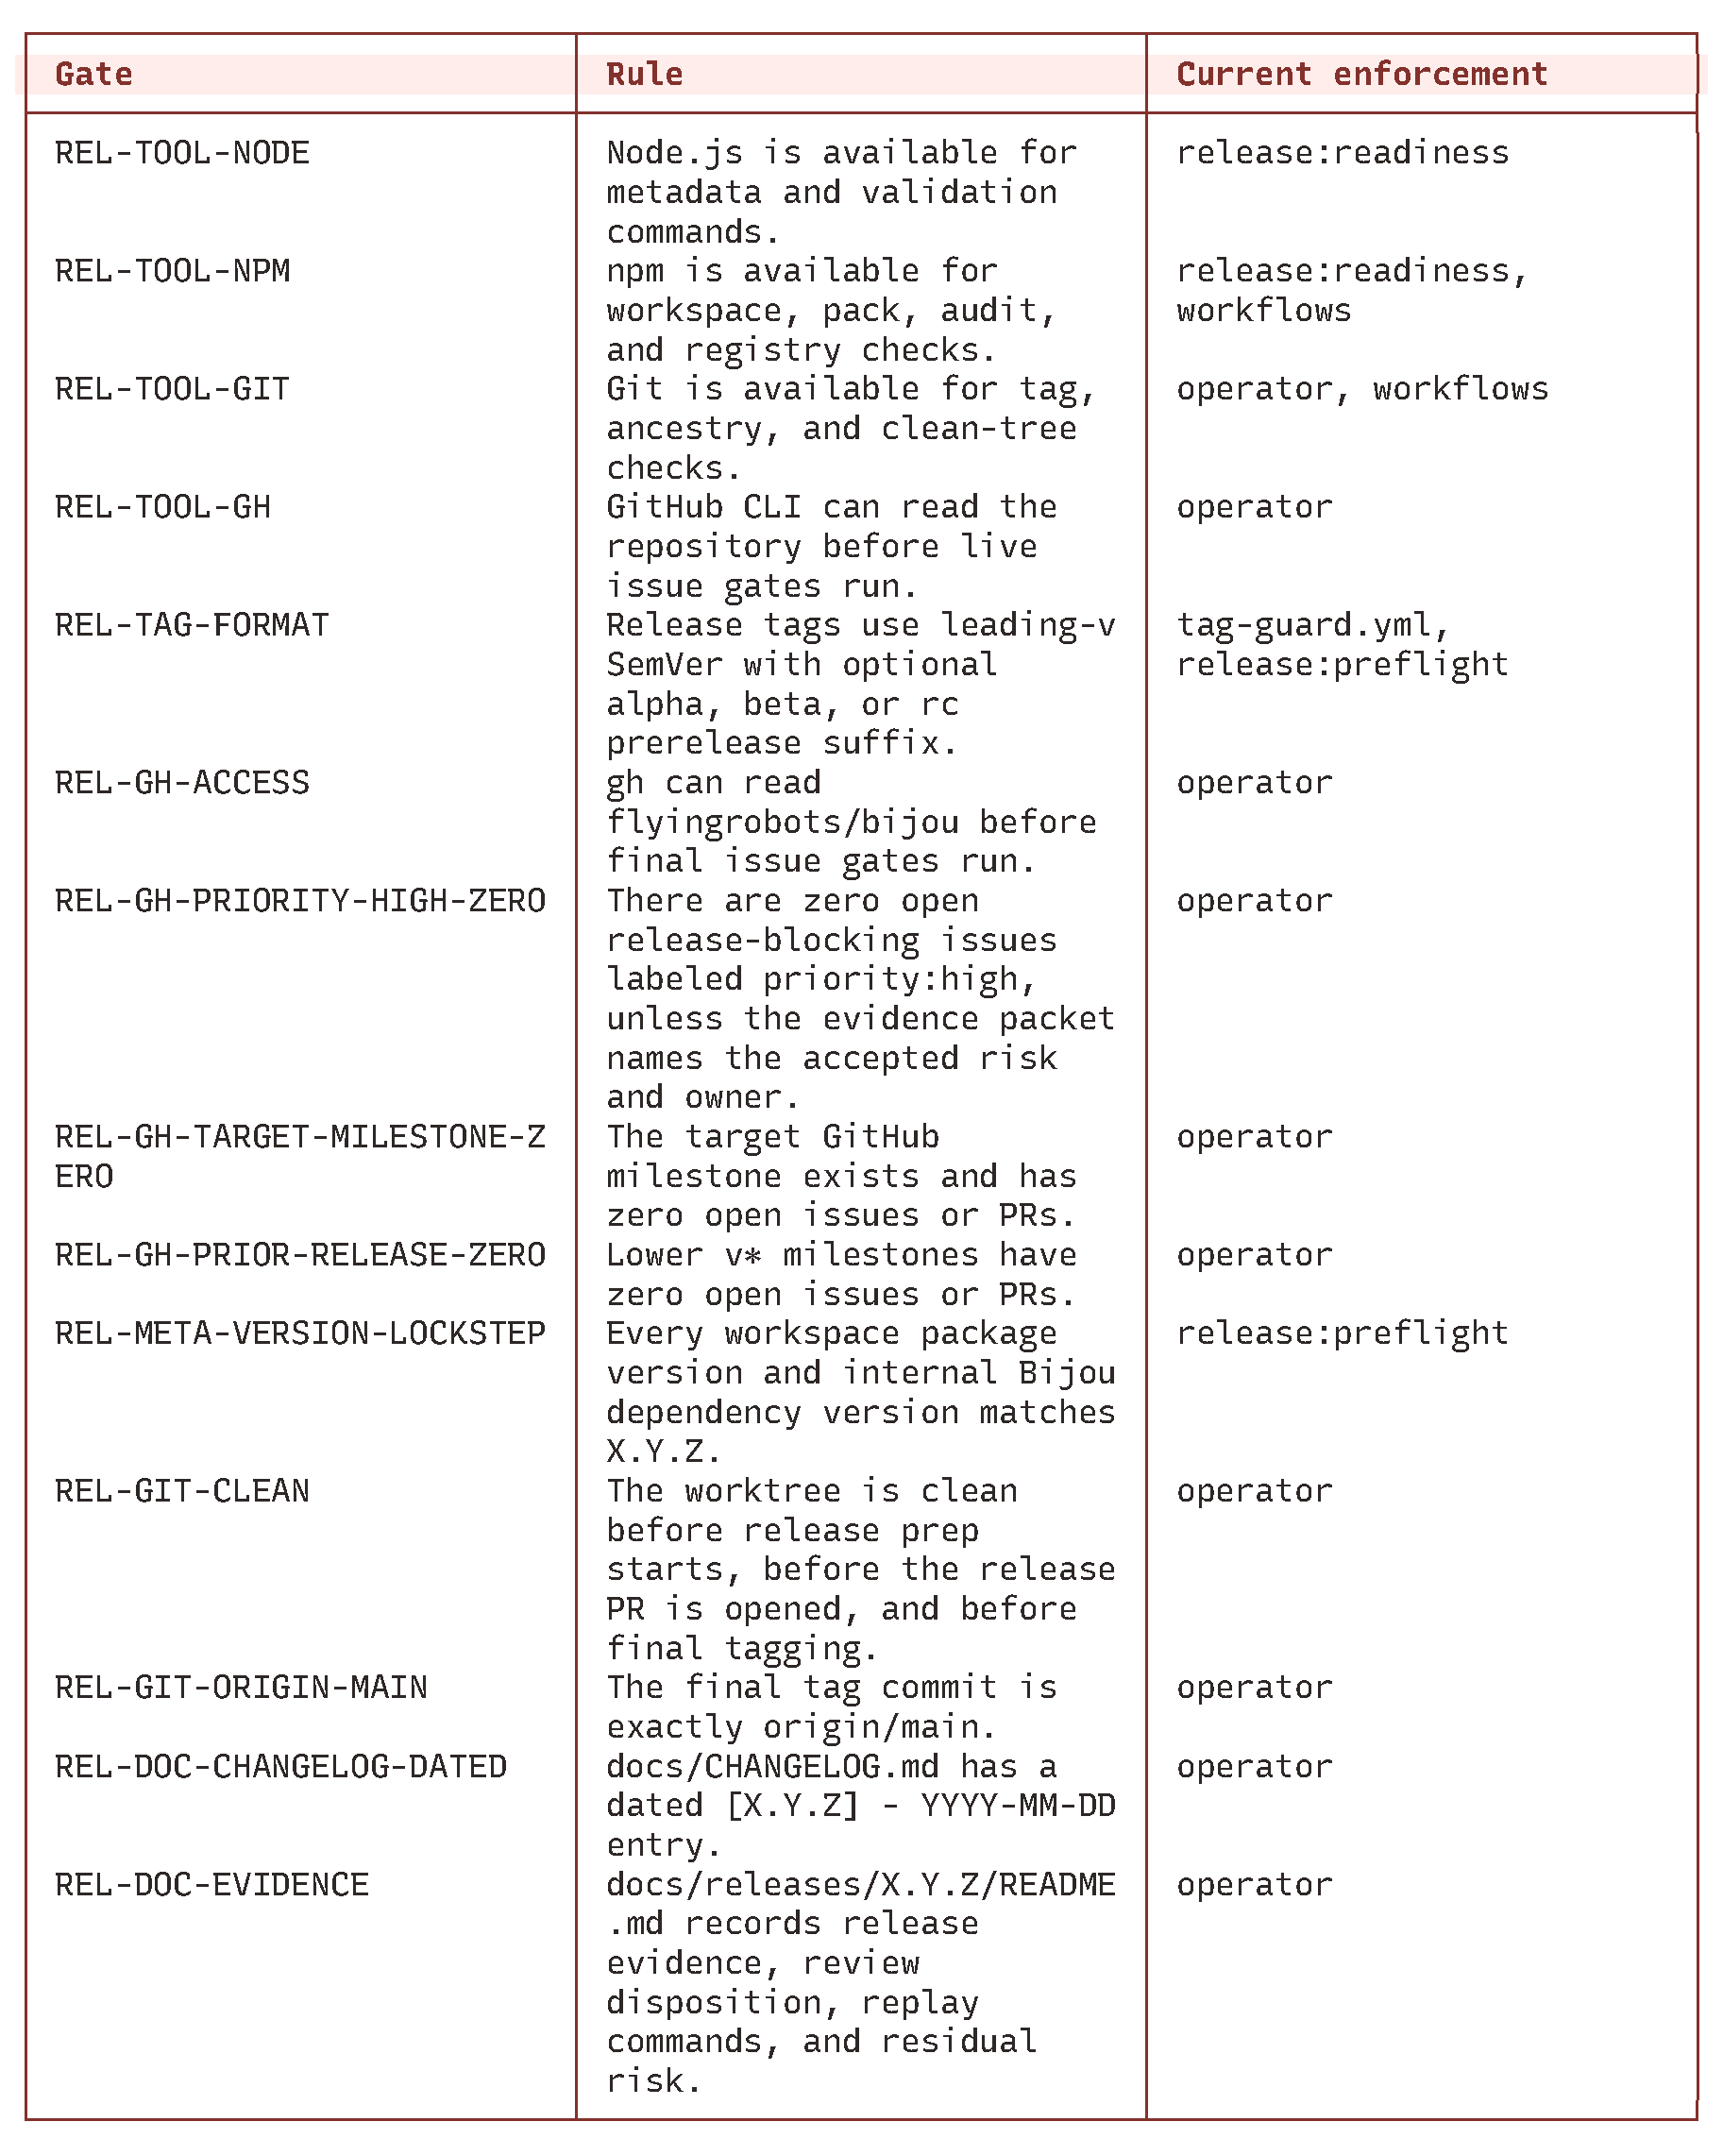
\includegraphics[width=\linewidth]{figures/tables/table-076-g1-1.pdf}
\par\smallskip{\scriptsize\color{BookMuted}Rows 1–14. Actual Bijou table component.}
\end{center}
\par\medskip
\begin{center}
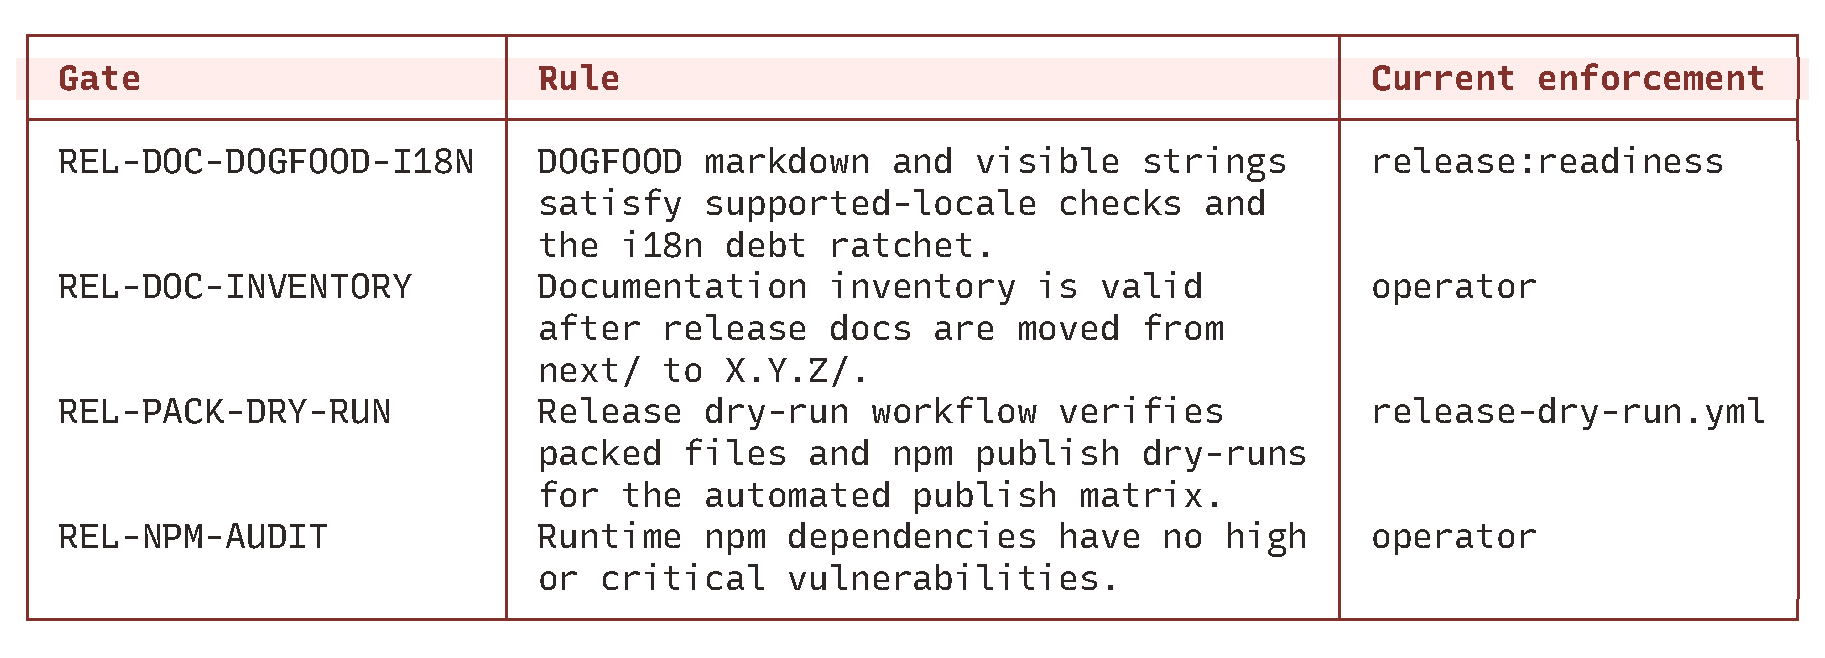
\includegraphics[width=\linewidth]{figures/tables/table-076-g1-2.pdf}
\par\smallskip{\scriptsize\color{BookMuted}Rows 15–18. Actual Bijou table component.}
\end{center}


The stage model is:

\begin{center}
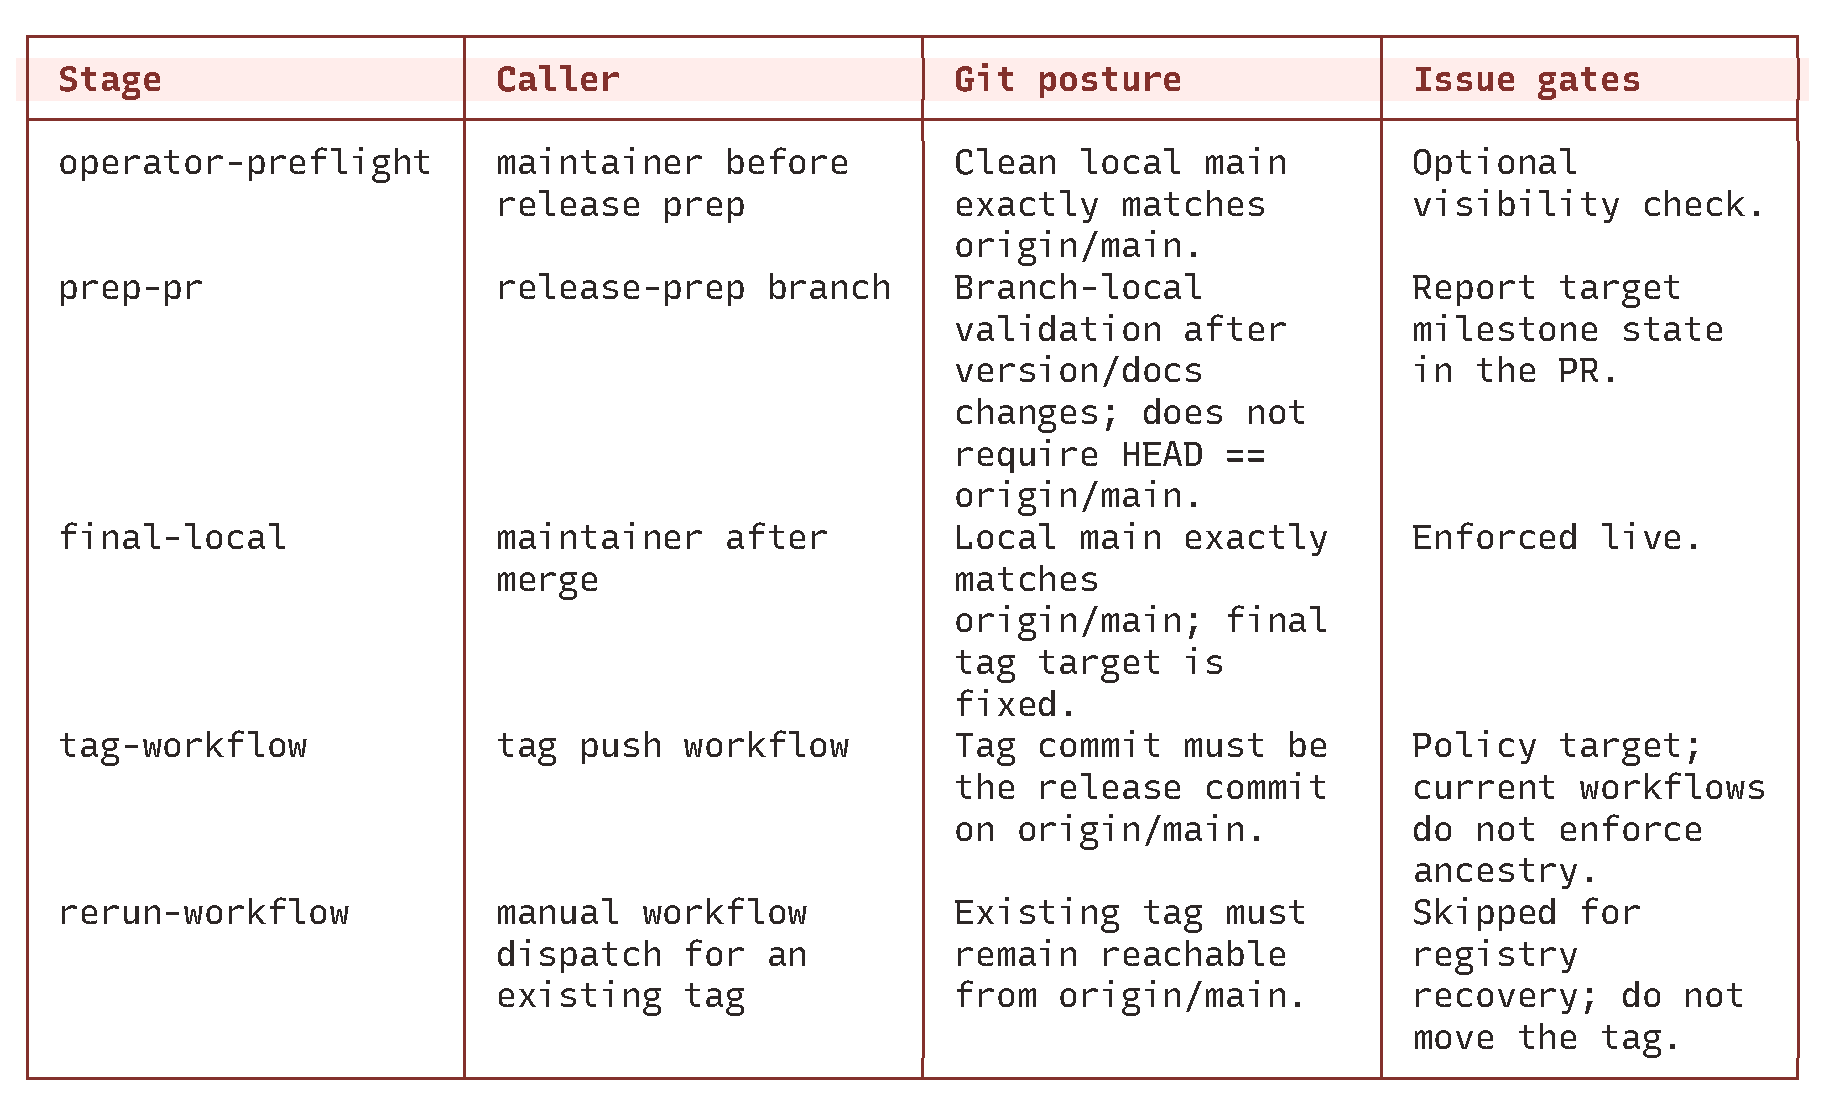
\includegraphics[width=\linewidth]{figures/tables/table-077-g1-1.pdf}
\par\smallskip{\scriptsize\color{BookMuted}Rows 1–5. Actual Bijou table component.}
\end{center}


\subsection{Human Review Gates}\label{record-274-human-review-gates}

Automation proves structure and repeatability. It does not prove release prose is truthful. The release evidence packet must record human review for:

\begin{itemize}
\tightlist
\item
  \texttt{d\allowbreak{}o\allowbreak{}c\allowbreak{}s\allowbreak{}/\allowbreak{}C\allowbreak{}H\allowbreak{}A\allowbreak{}N\allowbreak{}G\allowbreak{}E\allowbreak{}L\allowbreak{}O\allowbreak{}G\allowbreak{}.\allowbreak{}m\allowbreak{}d} accurately reflects the diff since the previous public tag.
\item
  \texttt{R\allowbreak{}E\allowbreak{}A\allowbreak{}D\allowbreak{}M\allowbreak{}E\allowbreak{}.\allowbreak{}m\allowbreak{}d} changed if front-door positioning, install commands, examples, or current release status changed.
\item
  \texttt{A\allowbreak{}R\allowbreak{}C\allowbreak{}H\allowbreak{}I\allowbreak{}T\allowbreak{}E\allowbreak{}C\allowbreak{}T\allowbreak{}U\allowbreak{}R\allowbreak{}E\allowbreak{}.\allowbreak{}m\allowbreak{}d} changed if ports, adapters, package boundaries, storage, rendering contracts, or runtime posture changed.
\item
  \texttt{d\allowbreak{}o\allowbreak{}c\allowbreak{}s\allowbreak{}/\allowbreak{}V\allowbreak{}I\allowbreak{}S\allowbreak{}I\allowbreak{}O\allowbreak{}N\allowbreak{}.\allowbreak{}m\allowbreak{}d}, \texttt{d\allowbreak{}o\allowbreak{}c\allowbreak{}s\allowbreak{}/\allowbreak{}W\allowbreak{}O\allowbreak{}R\allowbreak{}K\allowbreak{}F\allowbreak{}L\allowbreak{}O\allowbreak{}W\allowbreak{}.\allowbreak{}m\allowbreak{}d}, and GitHub milestone scope match the release posture; linked Linear items agree once migration is connected.
\item
  \texttt{d\allowbreak{}o\allowbreak{}c\allowbreak{}s\allowbreak{}/\allowbreak{}D\allowbreak{}O\allowbreak{}G\allowbreak{}F\allowbreak{}O\allowbreak{}O\allowbreak{}D\allowbreak{}.\allowbreak{}m\allowbreak{}d} and DOGFOOD-facing markdown changed if the docs app, release title, navigation model, localization posture, or proof surface changed.
\item
  Package READMEs, API references, migration docs, design-system docs, and MCP docs changed when their public surfaces changed.
\item
  Every landed release goalpost contributing to this version is named with its issue, design doc, landed PRs, completed slice count, deterministic proof, canonical fixtures or immutable inputs, witnesses, replay commands, and residual-risk disposition.
\item
  Any accepted residual risk is named with rationale, owner, and a follow-up issue. Hidden accepted failures are not allowed.
\end{itemize}

\subsection{Deterministic Reproducibility}\label{record-274-deterministic-reproducibility}

Evidence is complete only when another operator can replay it from the tag commit, committed release packet, and named immutable inputs.

Every release evidence packet must record:

\begin{itemize}
\tightlist
\item
  the exact command, script, workflow, or DOGFOOD route that produced each witness
\item
  the canonical fixture or immutable input used by that command, when the claim depends on more than repository state at the tag commit
\item
  the expected stable result, normalized output, digest, or screenshot assertion that replay must reproduce
\item
  any normalization applied for host-specific noise such as temp paths, clocks, terminal size, color mode, process IDs, registry timestamps, ordering, or environment-specific absolute paths
\end{itemize}

Place release-specific fixtures under \texttt{d\allowbreak{}o\allowbreak{}c\allowbreak{}s\allowbreak{}/\allowbreak{}r\allowbreak{}e\allowbreak{}l\allowbreak{}e\allowbreak{}a\allowbreak{}s\allowbreak{}e\allowbreak{}s\allowbreak{}/\allowbreak{}X\allowbreak{}.\allowbreak{}Y\allowbreak{}.\allowbreak{}Z\allowbreak{}/\allowbreak{}f\allowbreak{}i\allowbreak{}x\allowbreak{}t\allowbreak{}u\allowbreak{}r\allowbreak{}e\allowbreak{}s\allowbreak{}/} unless an existing committed fixture is already canonical. DOGFOOD terminal witnesses should record the route, command, terminal dimensions, shell theme or renderer mode, and stable assertion. A screenshot or recording is useful, but it is not a substitute for the command and immutable input that produced it.

\section{Current Release And Publish Surface}\label{record-274-current-release-and-publish-surface}

\subsection{Latest Shipped Release}\label{record-274-latest-shipped-release}

The latest shipped release is \textbf{\texttt{7\allowbreak{}.\allowbreak{}2\allowbreak{}.\allowbreak{}0}}.

\begin{itemize}
\tightlist
\item
  \texttt{7\allowbreak{}.\allowbreak{}2\allowbreak{}.\allowbreak{}0} - TUI mouse tracking and fallthrough stabilization, public page-scoped frame helpers, scripted mouse driver builders, DOGFOOD release story surfaces, Blocks app-binding snippets, theme and localization demo readiness, dependency audit cleanup, and Code Dojo ratchet progress
\item
  \texttt{7\allowbreak{}.\allowbreak{}1\allowbreak{}.\allowbreak{}0} - portable \texttt{u\allowbreak{}i\allowbreak{}-\allowbreak{}s\allowbreak{}c\allowbreak{}e\allowbreak{}n\allowbreak{}e\allowbreak{}-\allowbreak{}i\allowbreak{}r\allowbreak{}/\allowbreak{}1} proof, GraphQL-authored \texttt{b\allowbreak{}i\allowbreak{}j\allowbreak{}o\allowbreak{}u\allowbreak{}-\allowbreak{}b\allowbreak{}l\allowbreak{}o\allowbreak{}c\allowbreak{}k\allowbreak{}/\allowbreak{}1} artifacts, grouped debug facts, a real DOGFOOD NavigationListBlock fixture, terminal-rendering fixes, release-readiness guardrails, and DOGFOOD i18n debt coverage
\item
  \texttt{7\allowbreak{}.\allowbreak{}0\allowbreak{}.\allowbreak{}0} - DOGFOOD release identity, BlockLab naming, release-facing proof, theme/token work, image-to-glyph tooling, and V7 title-screen polish
\item
  \texttt{5\allowbreak{}.\allowbreak{}0\allowbreak{}.\allowbreak{}0} - frame-owned hosted runner, Node-host theme selection, crash-mode auto-exit, scoped Node I/O symlink hardening, deterministic scripted-example smoke, markdown pipe tables, and browsable-list marquee
\item
  \texttt{4\allowbreak{}.\allowbreak{}4\allowbreak{}.\allowbreak{}1} - framed-shell background-fill fixes, stock shell theme cycling, uppercase quit-confirm input
\item
  \texttt{4\allowbreak{}.\allowbreak{}4\allowbreak{}.\allowbreak{}0} - data-viz toolkit, zero-alloc framed app render, new bench scenarios
\item
  \texttt{4\allowbreak{}.\allowbreak{}3\allowbreak{}.\allowbreak{}0} - RE-008 byte-packed surface, RE-015 braille fix, \texttt{s\allowbreak{}e\allowbreak{}t\allowbreak{}R\allowbreak{}G\allowbreak{}B} API
\item
  \texttt{4\allowbreak{}.\allowbreak{}2\allowbreak{}.\allowbreak{}0} - RE-007 framed shell, \texttt{@\allowbreak{}f\allowbreak{}l\allowbreak{}y\allowbreak{}i\allowbreak{}n\allowbreak{}g\allowbreak{}r\allowbreak{}o\allowbreak{}b\allowbreak{}o\allowbreak{}t\allowbreak{}s\allowbreak{}/\allowbreak{}b\allowbreak{}i\allowbreak{}j\allowbreak{}o\allowbreak{}u\allowbreak{}-\allowbreak{}m\allowbreak{}c\allowbreak{}p}, METHOD migration
\item
  \texttt{4\allowbreak{}.\allowbreak{}1\allowbreak{}.\allowbreak{}0} - runtime engine through RE-006, DOGFOOD maturation (DF-021 through DF-026, including DF-023, DF-024, WF-003), i18n packages
\end{itemize}

The release smoke contract is DOGFOOD-centered through \texttt{s\allowbreak{}m\allowbreak{}o\allowbreak{}k\allowbreak{}e\allowbreak{}:\allowbreak{}d\allowbreak{}o\allowbreak{}g\allowbreak{}f\allowbreak{}o\allowbreak{}o\allowbreak{}d}, \texttt{s\allowbreak{}m\allowbreak{}o\allowbreak{}k\allowbreak{}e\allowbreak{}:\allowbreak{}d\allowbreak{}o\allowbreak{}g\allowbreak{}f\allowbreak{}o\allowbreak{}o\allowbreak{}d\allowbreak{}:\allowbreak{}l\allowbreak{}a\allowbreak{}n\allowbreak{}d\allowbreak{}i\allowbreak{}n\allowbreak{}g}, and \texttt{s\allowbreak{}m\allowbreak{}o\allowbreak{}k\allowbreak{}e\allowbreak{}:\allowbreak{}d\allowbreak{}o\allowbreak{}g\allowbreak{}f\allowbreak{}o\allowbreak{}o\allowbreak{}d\allowbreak{}:\allowbreak{}d\allowbreak{}o\allowbreak{}c\allowbreak{}s}.

Long-form release docs live under \texttt{d\allowbreak{}o\allowbreak{}c\allowbreak{}s\allowbreak{}/\allowbreak{}r\allowbreak{}e\allowbreak{}l\allowbreak{}e\allowbreak{}a\allowbreak{}s\allowbreak{}e\allowbreak{}s\allowbreak{}/\allowbreak{}<\allowbreak{}v\allowbreak{}e\allowbreak{}r\allowbreak{}s\allowbreak{}i\allowbreak{}o\allowbreak{}n\allowbreak{}>\allowbreak{}/}.

\subsection{Next Release Posture}\label{record-274-next-release-posture}

\texttt{8\allowbreak{}.\allowbreak{}0\allowbreak{}.\allowbreak{}0} is the next feature horizon: the Runtime Graph and Scene IR product contract built from the proof chain that \texttt{7\allowbreak{}.\allowbreak{}1\allowbreak{}.\allowbreak{}0} shipped and the release surface that \texttt{7\allowbreak{}.\allowbreak{}2\allowbreak{}.\allowbreak{}0} stabilized.

The latest shipped package release is \texttt{7\allowbreak{}.\allowbreak{}2\allowbreak{}.\allowbreak{}0}. The older \texttt{v\allowbreak{}6\allowbreak{}.\allowbreak{}0\allowbreak{}.\allowbreak{}0}, \texttt{v\allowbreak{}7\allowbreak{}.\allowbreak{}0\allowbreak{}.\allowbreak{}0}, \texttt{v\allowbreak{}7\allowbreak{}.\allowbreak{}1\allowbreak{}.\allowbreak{}0}, and \texttt{v\allowbreak{}7\allowbreak{}.\allowbreak{}2\allowbreak{}.\allowbreak{}0} milestones are zero-open tracker lanes retained as release lineage, not as the next target. The current target is the \texttt{v\allowbreak{}8\allowbreak{}.\allowbreak{}0\allowbreak{}.\allowbreak{}0} milestone.

Keep V8 limited to stable-release closeout. Do not reopen \texttt{7\allowbreak{}.\allowbreak{}2\allowbreak{}.\allowbreak{}0} for broad Theme Lab, BlockLab, localization workbench, VISOR, Geordi, or Runtime Graph product work.

Keep selected release scope in the \href{https://github.com/flyingrobots/bijou/milestone/6}{GitHub milestone} and proof in the versioned release packet. Stable \texttt{8\allowbreak{}.\allowbreak{}0\allowbreak{}.\allowbreak{}0} follows \texttt{8\allowbreak{}.\allowbreak{}0\allowbreak{}.\allowbreak{}0\allowbreak{}-\allowbreak{}r\allowbreak{}c\allowbreak{}.\allowbreak{}1}; \#526 owns version-lock enforcement and \#527 owns witness replay and documentation review. Linear execution migration is pending connection and workspace/team selection. Broad Sapphire and Theme Lab work remains in V9.

\subsection{Lock-step Versioned Units}\label{record-274-lock-step-versioned-units}

These workspaces move together:

\begin{itemize}
\tightlist
\item
  \texttt{@\allowbreak{}f\allowbreak{}l\allowbreak{}y\allowbreak{}i\allowbreak{}n\allowbreak{}g\allowbreak{}r\allowbreak{}o\allowbreak{}b\allowbreak{}o\allowbreak{}t\allowbreak{}s\allowbreak{}/\allowbreak{}b\allowbreak{}i\allowbreak{}j\allowbreak{}o\allowbreak{}u}
\item
  \texttt{@\allowbreak{}f\allowbreak{}l\allowbreak{}y\allowbreak{}i\allowbreak{}n\allowbreak{}g\allowbreak{}r\allowbreak{}o\allowbreak{}b\allowbreak{}o\allowbreak{}t\allowbreak{}s\allowbreak{}/\allowbreak{}b\allowbreak{}i\allowbreak{}j\allowbreak{}o\allowbreak{}u\allowbreak{}-\allowbreak{}n\allowbreak{}o\allowbreak{}d\allowbreak{}e}
\item
  \texttt{@\allowbreak{}f\allowbreak{}l\allowbreak{}y\allowbreak{}i\allowbreak{}n\allowbreak{}g\allowbreak{}r\allowbreak{}o\allowbreak{}b\allowbreak{}o\allowbreak{}t\allowbreak{}s\allowbreak{}/\allowbreak{}b\allowbreak{}i\allowbreak{}j\allowbreak{}o\allowbreak{}u\allowbreak{}-\allowbreak{}t\allowbreak{}u\allowbreak{}i}
\item
  \texttt{@\allowbreak{}f\allowbreak{}l\allowbreak{}y\allowbreak{}i\allowbreak{}n\allowbreak{}g\allowbreak{}r\allowbreak{}o\allowbreak{}b\allowbreak{}o\allowbreak{}t\allowbreak{}s\allowbreak{}/\allowbreak{}b\allowbreak{}i\allowbreak{}j\allowbreak{}o\allowbreak{}u\allowbreak{}-\allowbreak{}t\allowbreak{}u\allowbreak{}i\allowbreak{}-\allowbreak{}a\allowbreak{}p\allowbreak{}p}
\item
  \texttt{c\allowbreak{}r\allowbreak{}e\allowbreak{}a\allowbreak{}t\allowbreak{}e\allowbreak{}-\allowbreak{}b\allowbreak{}i\allowbreak{}j\allowbreak{}o\allowbreak{}u\allowbreak{}-\allowbreak{}t\allowbreak{}u\allowbreak{}i\allowbreak{}-\allowbreak{}a\allowbreak{}p\allowbreak{}p}
\item
  \texttt{@\allowbreak{}f\allowbreak{}l\allowbreak{}y\allowbreak{}i\allowbreak{}n\allowbreak{}g\allowbreak{}r\allowbreak{}o\allowbreak{}b\allowbreak{}o\allowbreak{}t\allowbreak{}s\allowbreak{}/\allowbreak{}b\allowbreak{}i\allowbreak{}j\allowbreak{}o\allowbreak{}u\allowbreak{}-\allowbreak{}i\allowbreak{}1\allowbreak{}8\allowbreak{}n}
\item
  \texttt{@\allowbreak{}f\allowbreak{}l\allowbreak{}y\allowbreak{}i\allowbreak{}n\allowbreak{}g\allowbreak{}r\allowbreak{}o\allowbreak{}b\allowbreak{}o\allowbreak{}t\allowbreak{}s\allowbreak{}/\allowbreak{}b\allowbreak{}i\allowbreak{}j\allowbreak{}o\allowbreak{}u\allowbreak{}-\allowbreak{}i\allowbreak{}1\allowbreak{}8\allowbreak{}n\allowbreak{}-\allowbreak{}t\allowbreak{}o\allowbreak{}o\allowbreak{}l\allowbreak{}s}
\item
  \texttt{@\allowbreak{}f\allowbreak{}l\allowbreak{}y\allowbreak{}i\allowbreak{}n\allowbreak{}g\allowbreak{}r\allowbreak{}o\allowbreak{}b\allowbreak{}o\allowbreak{}t\allowbreak{}s\allowbreak{}/\allowbreak{}b\allowbreak{}i\allowbreak{}j\allowbreak{}o\allowbreak{}u\allowbreak{}-\allowbreak{}i\allowbreak{}1\allowbreak{}8\allowbreak{}n\allowbreak{}-\allowbreak{}t\allowbreak{}o\allowbreak{}o\allowbreak{}l\allowbreak{}s\allowbreak{}-\allowbreak{}n\allowbreak{}o\allowbreak{}d\allowbreak{}e}
\item
  \texttt{@\allowbreak{}f\allowbreak{}l\allowbreak{}y\allowbreak{}i\allowbreak{}n\allowbreak{}g\allowbreak{}r\allowbreak{}o\allowbreak{}b\allowbreak{}o\allowbreak{}t\allowbreak{}s\allowbreak{}/\allowbreak{}b\allowbreak{}i\allowbreak{}j\allowbreak{}o\allowbreak{}u\allowbreak{}-\allowbreak{}i\allowbreak{}1\allowbreak{}8\allowbreak{}n\allowbreak{}-\allowbreak{}t\allowbreak{}o\allowbreak{}o\allowbreak{}l\allowbreak{}s\allowbreak{}-\allowbreak{}x\allowbreak{}l\allowbreak{}s\allowbreak{}x}
\item
  \texttt{@\allowbreak{}f\allowbreak{}l\allowbreak{}y\allowbreak{}i\allowbreak{}n\allowbreak{}g\allowbreak{}r\allowbreak{}o\allowbreak{}b\allowbreak{}o\allowbreak{}t\allowbreak{}s\allowbreak{}/\allowbreak{}b\allowbreak{}i\allowbreak{}j\allowbreak{}o\allowbreak{}u\allowbreak{}-\allowbreak{}m\allowbreak{}c\allowbreak{}p}
\item
  \texttt{@\allowbreak{}f\allowbreak{}l\allowbreak{}y\allowbreak{}i\allowbreak{}n\allowbreak{}g\allowbreak{}r\allowbreak{}o\allowbreak{}b\allowbreak{}o\allowbreak{}t\allowbreak{}s\allowbreak{}/\allowbreak{}b\allowbreak{}i\allowbreak{}j\allowbreak{}o\allowbreak{}u\allowbreak{}-\allowbreak{}b\allowbreak{}e\allowbreak{}n\allowbreak{}c\allowbreak{}h} (private benchmark workspace)
\end{itemize}

\subsection{Current Automated npm Publish Matrix}\label{record-274-current-automated-npm-publish-matrix}

As of now, the publish workflows automatically publish:

\begin{itemize}
\tightlist
\item
  \texttt{@\allowbreak{}f\allowbreak{}l\allowbreak{}y\allowbreak{}i\allowbreak{}n\allowbreak{}g\allowbreak{}r\allowbreak{}o\allowbreak{}b\allowbreak{}o\allowbreak{}t\allowbreak{}s\allowbreak{}/\allowbreak{}b\allowbreak{}i\allowbreak{}j\allowbreak{}o\allowbreak{}u}
\item
  \texttt{@\allowbreak{}f\allowbreak{}l\allowbreak{}y\allowbreak{}i\allowbreak{}n\allowbreak{}g\allowbreak{}r\allowbreak{}o\allowbreak{}b\allowbreak{}o\allowbreak{}t\allowbreak{}s\allowbreak{}/\allowbreak{}b\allowbreak{}i\allowbreak{}j\allowbreak{}o\allowbreak{}u\allowbreak{}-\allowbreak{}n\allowbreak{}o\allowbreak{}d\allowbreak{}e}
\item
  \texttt{@\allowbreak{}f\allowbreak{}l\allowbreak{}y\allowbreak{}i\allowbreak{}n\allowbreak{}g\allowbreak{}r\allowbreak{}o\allowbreak{}b\allowbreak{}o\allowbreak{}t\allowbreak{}s\allowbreak{}/\allowbreak{}b\allowbreak{}i\allowbreak{}j\allowbreak{}o\allowbreak{}u\allowbreak{}-\allowbreak{}t\allowbreak{}u\allowbreak{}i}
\item
  \texttt{@\allowbreak{}f\allowbreak{}l\allowbreak{}y\allowbreak{}i\allowbreak{}n\allowbreak{}g\allowbreak{}r\allowbreak{}o\allowbreak{}b\allowbreak{}o\allowbreak{}t\allowbreak{}s\allowbreak{}/\allowbreak{}b\allowbreak{}i\allowbreak{}j\allowbreak{}o\allowbreak{}u\allowbreak{}-\allowbreak{}t\allowbreak{}u\allowbreak{}i\allowbreak{}-\allowbreak{}a\allowbreak{}p\allowbreak{}p}
\item
  \texttt{c\allowbreak{}r\allowbreak{}e\allowbreak{}a\allowbreak{}t\allowbreak{}e\allowbreak{}-\allowbreak{}b\allowbreak{}i\allowbreak{}j\allowbreak{}o\allowbreak{}u\allowbreak{}-\allowbreak{}t\allowbreak{}u\allowbreak{}i\allowbreak{}-\allowbreak{}a\allowbreak{}p\allowbreak{}p}
\item
  \texttt{@\allowbreak{}f\allowbreak{}l\allowbreak{}y\allowbreak{}i\allowbreak{}n\allowbreak{}g\allowbreak{}r\allowbreak{}o\allowbreak{}b\allowbreak{}o\allowbreak{}t\allowbreak{}s\allowbreak{}/\allowbreak{}b\allowbreak{}i\allowbreak{}j\allowbreak{}o\allowbreak{}u\allowbreak{}-\allowbreak{}i\allowbreak{}1\allowbreak{}8\allowbreak{}n}
\item
  \texttt{@\allowbreak{}f\allowbreak{}l\allowbreak{}y\allowbreak{}i\allowbreak{}n\allowbreak{}g\allowbreak{}r\allowbreak{}o\allowbreak{}b\allowbreak{}o\allowbreak{}t\allowbreak{}s\allowbreak{}/\allowbreak{}b\allowbreak{}i\allowbreak{}j\allowbreak{}o\allowbreak{}u\allowbreak{}-\allowbreak{}i\allowbreak{}1\allowbreak{}8\allowbreak{}n\allowbreak{}-\allowbreak{}t\allowbreak{}o\allowbreak{}o\allowbreak{}l\allowbreak{}s}
\item
  \texttt{@\allowbreak{}f\allowbreak{}l\allowbreak{}y\allowbreak{}i\allowbreak{}n\allowbreak{}g\allowbreak{}r\allowbreak{}o\allowbreak{}b\allowbreak{}o\allowbreak{}t\allowbreak{}s\allowbreak{}/\allowbreak{}b\allowbreak{}i\allowbreak{}j\allowbreak{}o\allowbreak{}u\allowbreak{}-\allowbreak{}i\allowbreak{}1\allowbreak{}8\allowbreak{}n\allowbreak{}-\allowbreak{}t\allowbreak{}o\allowbreak{}o\allowbreak{}l\allowbreak{}s\allowbreak{}-\allowbreak{}n\allowbreak{}o\allowbreak{}d\allowbreak{}e}
\item
  \texttt{@\allowbreak{}f\allowbreak{}l\allowbreak{}y\allowbreak{}i\allowbreak{}n\allowbreak{}g\allowbreak{}r\allowbreak{}o\allowbreak{}b\allowbreak{}o\allowbreak{}t\allowbreak{}s\allowbreak{}/\allowbreak{}b\allowbreak{}i\allowbreak{}j\allowbreak{}o\allowbreak{}u\allowbreak{}-\allowbreak{}i\allowbreak{}1\allowbreak{}8\allowbreak{}n\allowbreak{}-\allowbreak{}t\allowbreak{}o\allowbreak{}o\allowbreak{}l\allowbreak{}s\allowbreak{}-\allowbreak{}x\allowbreak{}l\allowbreak{}s\allowbreak{}x}
\item
  \texttt{@\allowbreak{}f\allowbreak{}l\allowbreak{}y\allowbreak{}i\allowbreak{}n\allowbreak{}g\allowbreak{}r\allowbreak{}o\allowbreak{}b\allowbreak{}o\allowbreak{}t\allowbreak{}s\allowbreak{}/\allowbreak{}b\allowbreak{}i\allowbreak{}j\allowbreak{}o\allowbreak{}u\allowbreak{}-\allowbreak{}m\allowbreak{}c\allowbreak{}p}
\end{itemize}

\section{Phase 1: Repo Guards}\label{record-274-phase-1-repo-guards}

Run these checks before changing versions or docs.

\subsection{1. Clean worktree}\label{record-274-clean-worktree}

\begin{CodeBlock}
git status --porcelain=v1
\end{CodeBlock}

Abort if any output exists.

\subsection{2. Branch guard}\label{record-274-branch-guard}

\begin{CodeBlock}
git rev-parse --abbrev-ref HEAD
\end{CodeBlock}

Abort unless the result is \texttt{m\allowbreak{}a\allowbreak{}i\allowbreak{}n}.

\subsection{3. Sync with origin}\label{record-274-sync-with-origin}

\begin{CodeBlock}
git fetch origin main --tags --prune
git rev-parse HEAD origin/main
\end{CodeBlock}

Abort unless both SHAs are identical.

\subsection{4. Latest release tag}\label{record-274-latest-release-tag}

\begin{CodeBlock}
git tag --merged HEAD --list 'v*' --sort=-version:refname | head -n 1
\end{CodeBlock}

Abort if no valid release tag exists and there is no explicit first-release policy.

\section{Phase 2: Choose Version And Update Release Docs}\label{record-274-phase-2-choose-version-and-update-release-docs}

Bijou does \textbf{not} currently auto-compute the semver bump from commit history. The maintainer chooses the target version deliberately.

\subsection{0. Slice release-boundary work before the final PR}\label{record-274-slice-release-boundary-work-before-the-final-pr}

Before bumping versions, make sure feature and documentation work has already landed through reviewable precursor PRs.

Hard stop before opening a release-boundary PR:

\begin{itemize}
\tightlist
\item
  more than 140 changed files
\end{itemize}

Caution threshold:

\begin{itemize}
\tightlist
\item
  more than 10 commits
\item
  unrelated legends or cycle families on one branch
\item
  generated snapshots or docs mixed with unrelated runtime changes
\item
  more than one release-lane blocker implemented at once
\end{itemize}

When a threshold is hit, split the branch by cycle or product surface. The final release PR should primarily contain the version bump, changelog, long-form release docs, release-readiness proof, and final metadata updates.

\subsection{1. Pick the target version}\label{record-274-pick-the-target-version}

Allowed tag formats are:

\begin{itemize}
\tightlist
\item
  \texttt{v\allowbreak{}X\allowbreak{}.\allowbreak{}Y\allowbreak{}.\allowbreak{}Z}
\item
  \texttt{v\allowbreak{}X\allowbreak{}.\allowbreak{}Y\allowbreak{}.\allowbreak{}Z\allowbreak{}-\allowbreak{}r\allowbreak{}c\allowbreak{}.\allowbreak{}N}
\item
  \texttt{v\allowbreak{}X\allowbreak{}.\allowbreak{}Y\allowbreak{}.\allowbreak{}Z\allowbreak{}-\allowbreak{}b\allowbreak{}e\allowbreak{}t\allowbreak{}a\allowbreak{}.\allowbreak{}N}
\item
  \texttt{v\allowbreak{}X\allowbreak{}.\allowbreak{}Y\allowbreak{}.\allowbreak{}Z\allowbreak{}-\allowbreak{}a\allowbreak{}l\allowbreak{}p\allowbreak{}h\allowbreak{}a\allowbreak{}.\allowbreak{}N}
\end{itemize}

Stable releases should be the default unless there is a clear reason for a prerelease.

\subsection{2. Create the release-prep branch}\label{record-274-create-the-release-prep-branch}

Create the branch after the target version is known and before mutating files:

\begin{CodeBlock}
git switch -c release/vX.Y.Z
\end{CodeBlock}

For prereleases:

\begin{CodeBlock}
git switch -c release/vX.Y.Z-rc.N
\end{CodeBlock}

\subsection{3. Bump all workspace manifests}\label{record-274-bump-all-workspace-manifests}

\begin{CodeBlock}
npm run version X.Y.Z
\end{CodeBlock}

This updates all workspace package versions and pins internal dependency references to the exact same version.

\subsection{\texorpdfstring{4. Update \texttt{C\allowbreak{}H\allowbreak{}A\allowbreak{}N\allowbreak{}G\allowbreak{}E\allowbreak{}L\allowbreak{}O\allowbreak{}G\allowbreak{}.\allowbreak{}m\allowbreak{}d}}{4. Update }}\label{record-274-update-changelog.md}

\begin{itemize}
\tightlist
\item
  move \texttt{[\allowbreak{}U\allowbreak{}n\allowbreak{}r\allowbreak{}e\allowbreak{}l\allowbreak{}e\allowbreak{}a\allowbreak{}s\allowbreak{}e\allowbreak{}d\allowbreak{}]} into a real version header
\item
  use UTC date format \texttt{Y\allowbreak{}Y\allowbreak{}Y\allowbreak{}Y\allowbreak{}-\allowbreak{}M\allowbreak{}M\allowbreak{}-\allowbreak{}D\allowbreak{}D}
\item
  keep the existing changelog style intact
\item
  do not release with an empty \texttt{[\allowbreak{}U\allowbreak{}n\allowbreak{}r\allowbreak{}e\allowbreak{}l\allowbreak{}e\allowbreak{}a\allowbreak{}s\allowbreak{}e\allowbreak{}d\allowbreak{}]} section
\end{itemize}

\subsection{\texorpdfstring{5. Update \texttt{R\allowbreak{}E\allowbreak{}A\allowbreak{}D\allowbreak{}M\allowbreak{}E\allowbreak{}.\allowbreak{}m\allowbreak{}d}}{5. Update }}\label{record-274-update-readme.md}

\begin{itemize}
\tightlist
\item
  add or replace \texttt{\#\allowbreak{}\#\allowbreak{} \allowbreak{}W\allowbreak{}h\allowbreak{}a\allowbreak{}t\allowbreak{}'\allowbreak{}s\allowbreak{} \allowbreak{}N\allowbreak{}e\allowbreak{}w\allowbreak{} \allowbreak{}i\allowbreak{}n\allowbreak{} \allowbreak{}v\allowbreak{}X\allowbreak{}.\allowbreak{}Y\allowbreak{}.\allowbreak{}Z}
\item
  keep it concise and user-facing
\item
  keep a visible link to \href{https://github.com/flyingrobots/bijou/blob/cbd70612140e7a450d764b3c7be1c6af878b99bc/docs/CHANGELOG.md}{\texttt{C\allowbreak{}H\allowbreak{}A\allowbreak{}N\allowbreak{}G\allowbreak{}E\allowbreak{}L\allowbreak{}O\allowbreak{}G\allowbreak{}.\allowbreak{}m\allowbreak{}d}}
\end{itemize}

\subsection{6. Draft long-form release docs}\label{record-274-draft-long-form-release-docs}

Before the version is chosen, draft these in \texttt{d\allowbreak{}o\allowbreak{}c\allowbreak{}s\allowbreak{}/\allowbreak{}r\allowbreak{}e\allowbreak{}l\allowbreak{}e\allowbreak{}a\allowbreak{}s\allowbreak{}e\allowbreak{}s\allowbreak{}/\allowbreak{}n\allowbreak{}e\allowbreak{}x\allowbreak{}t\allowbreak{}/}:

\begin{itemize}
\tightlist
\item
  \texttt{R\allowbreak{}E\allowbreak{}A\allowbreak{}D\allowbreak{}M\allowbreak{}E\allowbreak{}.\allowbreak{}m\allowbreak{}d}
\item
  \texttt{w\allowbreak{}h\allowbreak{}a\allowbreak{}t\allowbreak{}s\allowbreak{}-\allowbreak{}n\allowbreak{}e\allowbreak{}w\allowbreak{}.\allowbreak{}m\allowbreak{}d}
\item
  \texttt{m\allowbreak{}i\allowbreak{}g\allowbreak{}r\allowbreak{}a\allowbreak{}t\allowbreak{}i\allowbreak{}o\allowbreak{}n\allowbreak{}-\allowbreak{}g\allowbreak{}u\allowbreak{}i\allowbreak{}d\allowbreak{}e\allowbreak{}.\allowbreak{}m\allowbreak{}d}
\end{itemize}

When the version is chosen, move that directory to \texttt{d\allowbreak{}o\allowbreak{}c\allowbreak{}s\allowbreak{}/\allowbreak{}r\allowbreak{}e\allowbreak{}l\allowbreak{}e\allowbreak{}a\allowbreak{}s\allowbreak{}e\allowbreak{}s\allowbreak{}/\allowbreak{}X\allowbreak{}.\allowbreak{}Y\allowbreak{}.\allowbreak{}Z\allowbreak{}/} and update any version placeholders inside the docs.

The versioned \texttt{R\allowbreak{}E\allowbreak{}A\allowbreak{}D\allowbreak{}M\allowbreak{}E\allowbreak{}.\allowbreak{}m\allowbreak{}d} is the release evidence packet. It must include:

\begin{itemize}
\tightlist
\item
  release summary
\item
  tracker and goalpost map
\item
  automated evidence matrix
\item
  human review matrix
\item
  deterministic reproducibility record
\item
  package and registry verification plan
\item
  residual-risk disposition
\end{itemize}

Historical releases before this policy may only have \texttt{w\allowbreak{}h\allowbreak{}a\allowbreak{}t\allowbreak{}s\allowbreak{}-\allowbreak{}n\allowbreak{}e\allowbreak{}w\allowbreak{}.\allowbreak{}m\allowbreak{}d} and \texttt{m\allowbreak{}i\allowbreak{}g\allowbreak{}r\allowbreak{}a\allowbreak{}t\allowbreak{}i\allowbreak{}o\allowbreak{}n\allowbreak{}-\allowbreak{}g\allowbreak{}u\allowbreak{}i\allowbreak{}d\allowbreak{}e\allowbreak{}.\allowbreak{}m\allowbreak{}d}. Future releases must carry the evidence packet.

\section{Phase 3: Local Validation}\label{record-274-phase-3-local-validation}

Run:

\begin{CodeBlock}
npm run release:preflight
npm run release:readiness -- --milestone vX.Y.Z
npm run docs:inventory
npm audit --omit=dev --audit-level=high
\end{CodeBlock}

\texttt{r\allowbreak{}e\allowbreak{}l\allowbreak{}e\allowbreak{}a\allowbreak{}s\allowbreak{}e\allowbreak{}:\allowbreak{}r\allowbreak{}e\allowbreak{}a\allowbreak{}d\allowbreak{}i\allowbreak{}n\allowbreak{}e\allowbreak{}s\allowbreak{}s} is the repo-native local gauntlet. With \texttt{-\allowbreak{}-\allowbreak{}m\allowbreak{}i\allowbreak{}l\allowbreak{}e\allowbreak{}s\allowbreak{}t\allowbreak{}o\allowbreak{}n\allowbreak{}e}, it first prints a release-readiness report and blocks before the gauntlet if:

\begin{itemize}
\tightlist
\item
  the target GitHub milestone has open tracker items, including issues or pull requests
\item
  any milestone tracker item still has \texttt{w\allowbreak{}o\allowbreak{}r\allowbreak{}k\allowbreak{}-\allowbreak{}i\allowbreak{}n\allowbreak{}-\allowbreak{}p\allowbreak{}r\allowbreak{}o\allowbreak{}g\allowbreak{}r\allowbreak{}e\allowbreak{}s\allowbreak{}s}
\item
  \texttt{C\allowbreak{}H\allowbreak{}A\allowbreak{}N\allowbreak{}G\allowbreak{}E\allowbreak{}L\allowbreak{}O\allowbreak{}G\allowbreak{}.\allowbreak{}m\allowbreak{}d} does not have an \texttt{U\allowbreak{}n\allowbreak{}r\allowbreak{}e\allowbreak{}l\allowbreak{}e\allowbreak{}a\allowbreak{}s\allowbreak{}e\allowbreak{}d} or versioned release boundary
\item
  \texttt{d\allowbreak{}o\allowbreak{}c\allowbreak{}s\allowbreak{}/\allowbreak{}r\allowbreak{}e\allowbreak{}l\allowbreak{}e\allowbreak{}a\allowbreak{}s\allowbreak{}e\allowbreak{}s\allowbreak{}/\allowbreak{}X\allowbreak{}.\allowbreak{}Y\allowbreak{}.\allowbreak{}Z\allowbreak{}/\allowbreak{}R\allowbreak{}E\allowbreak{}A\allowbreak{}D\allowbreak{}M\allowbreak{}E\allowbreak{}.\allowbreak{}m\allowbreak{}d} release evidence packet is missing
\item
  the command plan no longer includes package smoke or the release guide no longer documents the release dry-run package boundary
\end{itemize}

Without \texttt{-\allowbreak{}-\allowbreak{}m\allowbreak{}i\allowbreak{}l\allowbreak{}e\allowbreak{}s\allowbreak{}t\allowbreak{}o\allowbreak{}n\allowbreak{}e}, the command runs only the local gauntlet and does not require GitHub access. The gauntlet currently runs these gates in order:

\begin{enumerate}
\def\labelenumi{\arabic{enumi}.}
\tightlist
\item
  \texttt{b\allowbreak{}u\allowbreak{}i\allowbreak{}l\allowbreak{}d}
\item
  \texttt{l\allowbreak{}i\allowbreak{}n\allowbreak{}t}
\item
  \texttt{t\allowbreak{}y\allowbreak{}p\allowbreak{}e\allowbreak{}c\allowbreak{}h\allowbreak{}e\allowbreak{}c\allowbreak{}k\allowbreak{}:\allowbreak{}t\allowbreak{}e\allowbreak{}s\allowbreak{}t}
\item
  \texttt{d\allowbreak{}o\allowbreak{}c\allowbreak{}s\allowbreak{}:\allowbreak{}d\allowbreak{}e\allowbreak{}s\allowbreak{}i\allowbreak{}g\allowbreak{}n\allowbreak{}-\allowbreak{}s\allowbreak{}y\allowbreak{}s\allowbreak{}t\allowbreak{}e\allowbreak{}m\allowbreak{}:\allowbreak{}p\allowbreak{}r\allowbreak{}e\allowbreak{}f\allowbreak{}l\allowbreak{}i\allowbreak{}g\allowbreak{}h\allowbreak{}t}
\item
  \texttt{d\allowbreak{}o\allowbreak{}g\allowbreak{}f\allowbreak{}o\allowbreak{}o\allowbreak{}d\allowbreak{}:\allowbreak{}c\allowbreak{}o\allowbreak{}v\allowbreak{}e\allowbreak{}r\allowbreak{}a\allowbreak{}g\allowbreak{}e\allowbreak{}:\allowbreak{}g\allowbreak{}a\allowbreak{}t\allowbreak{}e}
\item
  \texttt{d\allowbreak{}o\allowbreak{}g\allowbreak{}f\allowbreak{}o\allowbreak{}o\allowbreak{}d\allowbreak{}:\allowbreak{}i\allowbreak{}1\allowbreak{}8\allowbreak{}n\allowbreak{}:\allowbreak{}c\allowbreak{}h\allowbreak{}e\allowbreak{}c\allowbreak{}k}
\item
  \texttt{d\allowbreak{}o\allowbreak{}g\allowbreak{}f\allowbreak{}o\allowbreak{}o\allowbreak{}d\allowbreak{}:\allowbreak{}i\allowbreak{}1\allowbreak{}8\allowbreak{}n\allowbreak{}:\allowbreak{}d\allowbreak{}e\allowbreak{}b\allowbreak{}t}
\item
  \texttt{w\allowbreak{}o\allowbreak{}r\allowbreak{}k\allowbreak{}f\allowbreak{}l\allowbreak{}o\allowbreak{}w\allowbreak{}:\allowbreak{}s\allowbreak{}h\allowbreak{}e\allowbreak{}l\allowbreak{}l\allowbreak{}:\allowbreak{}p\allowbreak{}r\allowbreak{}e\allowbreak{}f\allowbreak{}l\allowbreak{}i\allowbreak{}g\allowbreak{}h\allowbreak{}t}
\item
  \texttt{r\allowbreak{}e\allowbreak{}l\allowbreak{}e\allowbreak{}a\allowbreak{}s\allowbreak{}e\allowbreak{}:\allowbreak{}p\allowbreak{}r\allowbreak{}e\allowbreak{}f\allowbreak{}l\allowbreak{}i\allowbreak{}g\allowbreak{}h\allowbreak{}t}
\item
  \texttt{t\allowbreak{}e\allowbreak{}s\allowbreak{}t\allowbreak{}:\allowbreak{}f\allowbreak{}r\allowbreak{}a\allowbreak{}m\allowbreak{}e\allowbreak{}s}
\item
  \texttt{v\allowbreak{}e\allowbreak{}r\allowbreak{}i\allowbreak{}f\allowbreak{}y\allowbreak{}:\allowbreak{}i\allowbreak{}n\allowbreak{}t\allowbreak{}e\allowbreak{}r\allowbreak{}a\allowbreak{}c\allowbreak{}t\allowbreak{}i\allowbreak{}v\allowbreak{}e\allowbreak{}-\allowbreak{}e\allowbreak{}x\allowbreak{}a\allowbreak{}m\allowbreak{}p\allowbreak{}l\allowbreak{}e\allowbreak{}s}
\item
  \texttt{s\allowbreak{}m\allowbreak{}o\allowbreak{}k\allowbreak{}e\allowbreak{}:\allowbreak{}c\allowbreak{}a\allowbreak{}n\allowbreak{}a\allowbreak{}r\allowbreak{}i\allowbreak{}e\allowbreak{}s\allowbreak{} \allowbreak{}-\allowbreak{}-\allowbreak{} \allowbreak{}-\allowbreak{}-\allowbreak{}s\allowbreak{}k\allowbreak{}i\allowbreak{}p\allowbreak{}-\allowbreak{}b\allowbreak{}u\allowbreak{}i\allowbreak{}l\allowbreak{}d}
\item
  \texttt{s\allowbreak{}m\allowbreak{}o\allowbreak{}k\allowbreak{}e\allowbreak{}:\allowbreak{}d\allowbreak{}o\allowbreak{}g\allowbreak{}f\allowbreak{}o\allowbreak{}o\allowbreak{}d\allowbreak{} \allowbreak{}-\allowbreak{}-\allowbreak{} \allowbreak{}-\allowbreak{}-\allowbreak{}s\allowbreak{}k\allowbreak{}i\allowbreak{}p\allowbreak{}-\allowbreak{}b\allowbreak{}u\allowbreak{}i\allowbreak{}l\allowbreak{}d}
\item
  \texttt{n\allowbreak{}p\allowbreak{}m\allowbreak{} \allowbreak{}t\allowbreak{}e\allowbreak{}s\allowbreak{}t}
\end{enumerate}

Abort on any failure.

This reflects the current repo tooling after \href{https://github.com/flyingrobots/bijou/blob/cbd70612140e7a450d764b3c7be1c6af878b99bc/docs/design/WF-003-replace-smoke-examples-with-smoke-dogfood.md}{WF-003} moved the release smoke gate onto the DOGFOOD contract used for \texttt{4\allowbreak{}.\allowbreak{}1\allowbreak{}.\allowbreak{}0} and later releases.

\section{Phase 4: CI Dry Run}\label{record-274-phase-4-ci-dry-run}

Before tagging a real release, run the \textbf{Release Dry Run} workflow in GitHub Actions against the release-prep branch or PR commit.

This is currently the authoritative place where Bijou checks:

\begin{itemize}
\tightlist
\item
  packed file verification
\item
  npm publish dry-runs for the automated publish matrix
\item
  release notes preview generation
\end{itemize}

Until equivalent local tooling exists, treat the dry-run workflow as a required release gate for real releases.

\section{Phase 5: Commit, Push, And Open The Release PR}\label{record-274-phase-5-commit-push-and-open-the-release-pr}

After docs and validation are green:

\begin{CodeBlock}
git add -A
git commit -m "chore(release): vX.Y.Z"
git push -u origin release/vX.Y.Z
\end{CodeBlock}

For prereleases:

\begin{CodeBlock}
git commit -m "chore(release): vX.Y.Z-rc.N"
git push -u origin release/vX.Y.Z-rc.N
\end{CodeBlock}

Open a normal PR to \texttt{m\allowbreak{}a\allowbreak{}i\allowbreak{}n}. Do not open a draft PR. The PR body must link the release evidence packet, target milestone, changelog entry, release dry-run, and validation commands.

Merge the release PR only after review and green CI. Do not tag the branch commit before it is merged.

\section{Phase 6: Final Main Preflight And Tag}\label{record-274-phase-6-final-main-preflight-and-tag}

After the release PR is merged, fast-forward local \texttt{m\allowbreak{}a\allowbreak{}i\allowbreak{}n} to the exact release commit:

\begin{CodeBlock}
git fetch origin main --tags --prune
git switch main
git merge --ff-only origin/main
git status --porcelain=v1
git rev-parse HEAD origin/main
test "$(git rev-parse HEAD)" = "$(git rev-parse origin/main)"
npm run release:preflight
npm run docs:inventory
\end{CodeBlock}

Abort if the worktree is dirty, if the two printed SHAs differ, or if the \texttt{t\allowbreak{}e\allowbreak{}s\allowbreak{}t} command fails. Local \texttt{m\allowbreak{}a\allowbreak{}i\allowbreak{}n} must exactly match \texttt{o\allowbreak{}r\allowbreak{}i\allowbreak{}g\allowbreak{}i\allowbreak{}n\allowbreak{}/\allowbreak{}m\allowbreak{}a\allowbreak{}i\allowbreak{}n}; being ahead of \texttt{o\allowbreak{}r\allowbreak{}i\allowbreak{}g\allowbreak{}i\allowbreak{}n\allowbreak{}/\allowbreak{}m\allowbreak{}a\allowbreak{}i\allowbreak{}n} is also release-blocking.

Create the tag from that exact commit:

\begin{CodeBlock}
git tag -a vX.Y.Z -m "release: vX.Y.Z"
\end{CodeBlock}

For prereleases:

\begin{CodeBlock}
git tag -a vX.Y.Z-rc.N -m "release: vX.Y.Z-rc.N"
\end{CodeBlock}

Bijou currently enforces tag \textbf{format} through \href{https://github.com/flyingrobots/bijou/blob/cbd70612140e7a450d764b3c7be1c6af878b99bc/.github/workflows/tag-guard.yml}{tag-guard.yml}, not signed tags. Do not pretend signed-tag policy exists unless the automation is updated to require it.

\section{Phase 7: Push The Tag And Let Automation Publish}\label{record-274-phase-7-push-the-tag-and-let-automation-publish}

Push only the tag:

\begin{CodeBlock}
git push origin vX.Y.Z
\end{CodeBlock}

The publish workflow then owns:

\begin{itemize}
\tightlist
\item
  metadata verification
\item
  build, lint, typecheck, test, smoke, and packed-file verification
\item
  npm publication for the automated publish matrix
\item
  GitHub Release creation or update
\end{itemize}

If a tag has already been pushed and the publish workflow itself needs a repair, fix \texttt{.\allowbreak{}g\allowbreak{}i\allowbreak{}t\allowbreak{}h\allowbreak{}u\allowbreak{}b\allowbreak{}/\allowbreak{}w\allowbreak{}o\allowbreak{}r\allowbreak{}k\allowbreak{}f\allowbreak{}l\allowbreak{}o\allowbreak{}w\allowbreak{}s\allowbreak{}/\allowbreak{}p\allowbreak{}u\allowbreak{}b\allowbreak{}l\allowbreak{}i\allowbreak{}s\allowbreak{}h\allowbreak{}.\allowbreak{}y\allowbreak{}m\allowbreak{}l} on \texttt{m\allowbreak{}a\allowbreak{}i\allowbreak{}n} and then rerun the same release through the workflow's \texttt{w\allowbreak{}o\allowbreak{}r\allowbreak{}k\allowbreak{}f\allowbreak{}l\allowbreak{}o\allowbreak{}w\allowbreak{}\_\allowbreak{}d\allowbreak{}i\allowbreak{}s\allowbreak{}p\allowbreak{}a\allowbreak{}t\allowbreak{}c\allowbreak{}h} entrypoint using the existing tag and release ref. Do not delete or move the release tag just to recover from workflow drift.

Do not manually create a GitHub Release unless the automation fails and the process is being explicitly repaired.

\section{Phase 8: Verify The Result}\label{record-274-phase-8-verify-the-result}

Do not stop at ``workflow started.''

Verify all of the following:

\begin{itemize}
\tightlist
\item
  the tag-guard workflow passed
\item
  the publish workflow passed
\item
  npm shows the new version for each package in the automated publish matrix
\item
  npm dist-tags match the release type

  \begin{itemize}
  \tightlist
  \item
    stable -\textgreater{} \texttt{l\allowbreak{}a\allowbreak{}t\allowbreak{}e\allowbreak{}s\allowbreak{}t}
  \item
    \texttt{r\allowbreak{}c} -\textgreater{} \texttt{n\allowbreak{}e\allowbreak{}x\allowbreak{}t}
  \item
    \texttt{b\allowbreak{}e\allowbreak{}t\allowbreak{}a} -\textgreater{} \texttt{b\allowbreak{}e\allowbreak{}t\allowbreak{}a}
  \item
    \texttt{a\allowbreak{}l\allowbreak{}p\allowbreak{}h\allowbreak{}a} -\textgreater{} \texttt{a\allowbreak{}l\allowbreak{}p\allowbreak{}h\allowbreak{}a}
  \end{itemize}
\item
  the GitHub Release exists with the expected notes
\end{itemize}

Representative checks:

\begin{CodeBlock}
npm view @flyingrobots/bijou version dist-tags --json
npm view @flyingrobots/bijou-node version dist-tags --json
npm view @flyingrobots/bijou-tui version dist-tags --json
npm view @flyingrobots/bijou-tui-app version dist-tags --json
npm view create-bijou-tui-app version dist-tags --json
npm view @flyingrobots/bijou-i18n version dist-tags --json
npm view @flyingrobots/bijou-i18n-tools version dist-tags --json
npm view @flyingrobots/bijou-i18n-tools-node version dist-tags --json
npm view @flyingrobots/bijou-i18n-tools-xlsx version dist-tags --json
npm view @flyingrobots/bijou-mcp version dist-tags --json
\end{CodeBlock}

\section{Abort Conditions}\label{record-274-abort-conditions}

Abort immediately if any of these are true:

\begin{itemize}
\tightlist
\item
  Phase 1 preflight starts from a dirty worktree
\item
  Phase 1 preflight starts with the operator checked out to a branch other than \texttt{m\allowbreak{}a\allowbreak{}i\allowbreak{}n}; after Phase 1 passes, Phase 2 step 2 creates the \texttt{r\allowbreak{}e\allowbreak{}l\allowbreak{}e\allowbreak{}a\allowbreak{}s\allowbreak{}e\allowbreak{}/\allowbreak{}v\allowbreak{}X\allowbreak{}.\allowbreak{}Y\allowbreak{}.\allowbreak{}Z} branch where prep work continues
\item
  final tag prep is not on \texttt{m\allowbreak{}a\allowbreak{}i\allowbreak{}n}
\item
  final tag prep is not exactly synced to \texttt{o\allowbreak{}r\allowbreak{}i\allowbreak{}g\allowbreak{}i\allowbreak{}n\allowbreak{}/\allowbreak{}m\allowbreak{}a\allowbreak{}i\allowbreak{}n}
\item
  version bump not reflected cleanly across the workspace
\item
  \texttt{C\allowbreak{}H\allowbreak{}A\allowbreak{}N\allowbreak{}G\allowbreak{}E\allowbreak{}L\allowbreak{}O\allowbreak{}G\allowbreak{}.\allowbreak{}m\allowbreak{}d} still has no real release section
\item
  \texttt{d\allowbreak{}o\allowbreak{}c\allowbreak{}s\allowbreak{}/\allowbreak{}r\allowbreak{}e\allowbreak{}l\allowbreak{}e\allowbreak{}a\allowbreak{}s\allowbreak{}e\allowbreak{}s\allowbreak{}/\allowbreak{}X\allowbreak{}.\allowbreak{}Y\allowbreak{}.\allowbreak{}Z\allowbreak{}/\allowbreak{}R\allowbreak{}E\allowbreak{}A\allowbreak{}D\allowbreak{}M\allowbreak{}E\allowbreak{}.\allowbreak{}m\allowbreak{}d} release evidence packet is missing
\item
  target GitHub milestone does not exist
\item
  target GitHub milestone has open issues or PRs
\item
  lower \texttt{v\allowbreak{}*} GitHub milestones have open issues or PRs
\item
  open \texttt{p\allowbreak{}r\allowbreak{}i\allowbreak{}o\allowbreak{}r\allowbreak{}i\allowbreak{}t\allowbreak{}y\allowbreak{}:\allowbreak{}h\allowbreak{}i\allowbreak{}g\allowbreak{}h} issues lack an explicit release-risk disposition
\item
  \texttt{r\allowbreak{}e\allowbreak{}l\allowbreak{}e\allowbreak{}a\allowbreak{}s\allowbreak{}e\allowbreak{}:\allowbreak{}p\allowbreak{}r\allowbreak{}e\allowbreak{}f\allowbreak{}l\allowbreak{}i\allowbreak{}g\allowbreak{}h\allowbreak{}t} fails
\item
  \texttt{r\allowbreak{}e\allowbreak{}l\allowbreak{}e\allowbreak{}a\allowbreak{}s\allowbreak{}e\allowbreak{}:\allowbreak{}r\allowbreak{}e\allowbreak{}a\allowbreak{}d\allowbreak{}i\allowbreak{}n\allowbreak{}e\allowbreak{}s\allowbreak{}s} fails
\item
  \texttt{d\allowbreak{}o\allowbreak{}c\allowbreak{}s\allowbreak{}:\allowbreak{}i\allowbreak{}n\allowbreak{}v\allowbreak{}e\allowbreak{}n\allowbreak{}t\allowbreak{}o\allowbreak{}r\allowbreak{}y} fails
\item
  \texttt{n\allowbreak{}p\allowbreak{}m\allowbreak{} \allowbreak{}a\allowbreak{}u\allowbreak{}d\allowbreak{}i\allowbreak{}t\allowbreak{} \allowbreak{}-\allowbreak{}-\allowbreak{}o\allowbreak{}m\allowbreak{}i\allowbreak{}t\allowbreak{}=\allowbreak{}d\allowbreak{}e\allowbreak{}v\allowbreak{} \allowbreak{}-\allowbreak{}-\allowbreak{}a\allowbreak{}u\allowbreak{}d\allowbreak{}i\allowbreak{}t\allowbreak{}-\allowbreak{}l\allowbreak{}e\allowbreak{}v\allowbreak{}e\allowbreak{}l\allowbreak{}=\allowbreak{}h\allowbreak{}i\allowbreak{}g\allowbreak{}h} fails
\item
  release dry-run fails
\item
  tag push fails
\item
  publish workflow fails
\item
  npm does not show the new version and expected dist-tag mapping
\end{itemize}

\section{Known Current Gaps}\label{record-274-known-current-gaps}

\begin{itemize}
\tightlist
\item
  Bijou does not yet have a stage-aware \texttt{r\allowbreak{}e\allowbreak{}l\allowbreak{}e\allowbreak{}a\allowbreak{}s\allowbreak{}e\allowbreak{}:\allowbreak{}p\allowbreak{}r\allowbreak{}e\allowbreak{}p} or \texttt{r\allowbreak{}e\allowbreak{}l\allowbreak{}e\allowbreak{}a\allowbreak{}s\allowbreak{}e\allowbreak{}:\allowbreak{}g\allowbreak{}u\allowbreak{}a\allowbreak{}r\allowbreak{}d} script. The policy names those gates, but \texttt{r\allowbreak{}e\allowbreak{}l\allowbreak{}e\allowbreak{}a\allowbreak{}s\allowbreak{}e\allowbreak{}:\allowbreak{}p\allowbreak{}r\allowbreak{}e\allowbreak{}f\allowbreak{}l\allowbreak{}i\allowbreak{}g\allowbreak{}h\allowbreak{}t} and \texttt{r\allowbreak{}e\allowbreak{}l\allowbreak{}e\allowbreak{}a\allowbreak{}s\allowbreak{}e\allowbreak{}:\allowbreak{}r\allowbreak{}e\allowbreak{}a\allowbreak{}d\allowbreak{}i\allowbreak{}n\allowbreak{}e\allowbreak{}s\allowbreak{}s} are the current repo-native commands.
\item
  clean-worktree is an operator preflight check, not a \texttt{r\allowbreak{}e\allowbreak{}l\allowbreak{}e\allowbreak{}a\allowbreak{}s\allowbreak{}e\allowbreak{}:\allowbreak{}r\allowbreak{}e\allowbreak{}a\allowbreak{}d\allowbreak{}i\allowbreak{}n\allowbreak{}e\allowbreak{}s\allowbreak{}s} concern, because Phase 2 intentionally dirties the worktree
\item
  branch-sync, latest-tag, tag-collision, live GitHub pull-request milestone gates, changelog dating, release tag ancestry, release evidence shape, and human review disposition are documented here, but they do not yet have a single dedicated repo-native guard
\item
  \texttt{d\allowbreak{}o\allowbreak{}c\allowbreak{}s\allowbreak{}:\allowbreak{}i\allowbreak{}n\allowbreak{}v\allowbreak{}e\allowbreak{}n\allowbreak{}t\allowbreak{}o\allowbreak{}r\allowbreak{}y} and runtime \texttt{n\allowbreak{}p\allowbreak{}m\allowbreak{} \allowbreak{}a\allowbreak{}u\allowbreak{}d\allowbreak{}i\allowbreak{}t} are release policy gates but are not currently part of \texttt{r\allowbreak{}e\allowbreak{}l\allowbreak{}e\allowbreak{}a\allowbreak{}s\allowbreak{}e\allowbreak{}:\allowbreak{}r\allowbreak{}e\allowbreak{}a\allowbreak{}d\allowbreak{}i\allowbreak{}n\allowbreak{}e\allowbreak{}s\allowbreak{}s}
\item
  JSR publishing is not currently part of Bijou's release surface
\item
  signed tags are not currently a repo policy
\end{itemize}

If any of those policies change, update this doc and the automation together.

